\chapter{Objašnjenja korištenih pojmova}

Prije opisa postojećih metoda detekcije objekata potrebno je objasniti često korištene pojmove prilikom detektiranja objekata 

\section{mAP vrijednost}

Ova vrijednost predstavlja srednju vrijednost srednjih preciznosti svih razreda nad svim \newline 
vrijednostima IoU iz skupa podataka i koristi se prilikom evaluiranja točnosti treniranog modela. 
Kako bi se mogla objasniti vrijednost i značenje mAPa prilikom validacije nekog modela, prvo se moraju objasniti pojmovi
preciznosti \engl{precission} i opoziva \engl{recall}. Preciznost je omjer uspješno klasificiranih objekata i svih klasificiranih objekata na slici. 
Opoziv je omjer broja uspješno klasificiranih objekata i stvarnog broja objekata tražene klase na slici. 
Srednja preciznost \engl{Average precision} je srednja vrijednost maksimalne preciznosti za vrijednosti opoziva između 0 i 1 s korakom 
od 0.1. U nastavku će srednja preciznost biti označena oznakom SP. \newline 
Formulom  $SP=\frac{1}{11}\sum_{n=0}^{10} P(R(n))$ računa se ova vrijednost. R(n) označava n-tu vrijednosti opoziva iz polja [0, 0.1, 0.2, ... , 1.0], a 
P(R(n)) je vrijednost maksimalne preciznosti za R(n). \citep{everingham2010pascal}

Ove vrijednosti pokazuju točnost modela prilikom klasificiranja objekata na slikama. Uz ove vrijednosti potrebno je odrediti odrediti i uspješnost modela prilikom lokalizacije, tj. 
određivanja pozicije na slici gdje se objekt nalazi. Za ovu vrijednost potrebno je izračunati IoU \engl{Intersect over union} ili omjer presjeka i unije okvira temeljne istine i 
generiranog okvira. Okvir temeljne istine je pravokutnik koji omeđuje objekt na slici i može biti zapisan u različitim formatima. Na primjer, može biti u formatu 
[x\_min, y\_min, x\_max, y\_max] ili [x\_središte, y\_središte, širina, visina]. Okviri temeljne istine unose se ručno za svaku fotografiju u skupu. \newline

Vizualni prikaz računanja vrijednosti IoU nalazi se na slici ~\ref{IoU}

\begin{figure}[htb]
    \centering
    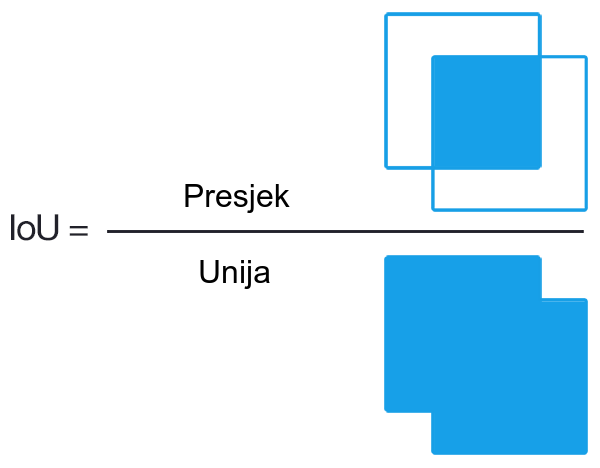
\includegraphics[width=8cm]{img/iou_equation.png}
    \caption{Omjer presjeka i unije}
    \label{IoU}
\end{figure}

Za računanje mAPa može se uzeti jedna vrijednost IoU koja predstavlja granicu. Rezultati detektiranja kojima je IoU manji od ove vrijednosti se odbacuju.
Ostalim rezultatima računa se SP. mAP je rezultat izračuna srednje vrijednosti SPa svih razreda. Može se također uzeti skup vrijednosti IoU koje predstavljaju granicu. 
Skup vrijednosti može biti proizvoljan, ali se na primjer za COCO natjecanja uzima skup vrijednosti između 0.5 i 0.95 uz korak 0.05. \footnote{\url{http://cocodataset.org/\#detection-eval}}